\begin{enumerate}[label=\thechapter.\arabic*,ref=\thechapter.\theenumi]

\item The damping ratio and undamped natural frequency of a closed loop system as
shown in the figure, are denoted as $\zeta$ and $\omega_n$, respectively. The values of $\zeta$ and $\omega_n$
are 
\begin{figure}[!ht]
\centering
\begin{center}
\includegraphics[width=\columnwidth]{2022/EE/39/figs/question.jpg}
\end{center}
%\caption{Diagram for GATE ME Question 30}
\end{figure}
\begin{enumerate}
    \item $\zeta = 0.5$ and $\omega_n = 10$ rad/s
    \item $\zeta = 0.1$ and $\omega_n = 10$ rad/s
    \item $\zeta = 0.707$ and $\omega_n = 10$ rad/s
    \item $\zeta = 0.707$ and $\omega_n = 100$ rad/s
\end{enumerate}
\hfill(GATE EE 2022)
\solution
\iffalse
\let\negmedspace\undefined
\let\negthickspace\undefined
\documentclass[journal,12pt,twocolumn]{IEEEtran}
\usepackage{cite}
\usepackage{amsmath,amssymb,amsfonts,amsthm}
\usepackage{algorithmic}
\usepackage{graphicx}
\usepackage{textcomp}
\usepackage{xcolor}
\usepackage{txfonts}
\usepackage{listings}
\usepackage{enumitem}
\usepackage{mathtools}
\usepackage{gensymb}
\usepackage{comment}
\usepackage[breaklinks=true]{hyperref}
\usepackage{tkz-euclide} 
\usepackage{listings}
\usepackage{gvv}                                        
\def\inputGnumericTable{}                                 
\usepackage[latin1]{inputenc}                                
\usepackage{color}                                            
\usepackage{array}                                            
\usepackage{longtable}                                       
\usepackage{calc}                                             
\usepackage{multirow}                                         
\usepackage{hhline}                                           
\usepackage{ifthen}                                           
\usepackage{lscape}
\usepackage{placeins}
\usepackage{xparse}


\newtheorem{theorem}{Theorem}[section]
\newtheorem{problem}{Problem}
\newtheorem{proposition}{Proposition}[section]
\newtheorem{lemma}{Lemma}[section]
\newtheorem{corollary}[theorem]{Corollary}
\newtheorem{example}{Example}[section]
\newtheorem{definition}[problem]{Definition}
\newcommand{\BEQA}{\begin{eqnarray}}
\newcommand{\EEQA}{\end{eqnarray}}
\newcommand{\define}{\stackrel{\triangle}{=}}
\theoremstyle{remark}
\newtheorem{rem}{Remark}

\graphicspath{ {./figs/} } 

\begin{document}

\bibliographystyle{IEEEtran}
\vspace{3cm}

\Large\title{GATE 2022 EE 39}
\large\author{EE23BTECH11032 - Kaustubh Parag Khachane $^{*}$% <-this % stops a space
}
\maketitle
\newpage
\bigskip

\renewcommand{\thefigure}{\theenumi}
\renewcommand{\thetable}{\theenumi}
\large\textbf{Question GATE 22 EE 39} :\\
The damping ratio and undamped natural frequency of a closed loop system as
shown in the figure, are denoted as $\zeta$ and $\omega_n$, respectively. The values of $\zeta$ and $\omega_n$
are 
\begin{figure}[!ht]
\centering
\begin{center}
\includegraphics[width=\columnwidth]{question}
\end{center}
%\caption{Diagram for GATE ME Question 30}
\end{figure}
\begin{enumerate}
    \item $\zeta = 0.5$ and $\omega_n = 10$ rad/s
    \item $\zeta = 0.1$ and $\omega_n = 10$ rad/s
    \item $\zeta = 0.707$ and $\omega_n = 10$ rad/s
    \item $\zeta = 0.707$ and $\omega_n = 100$ rad/s
\end{enumerate}
\hfill(GATE EE 2022)\\
\solution\\
\fi
\begin{table}[!ht] 
\centering
\setlength{\extrarowheight}{8pt}
\begin{tabular}{|l|l|l|}
    \hline
    \textbf{Parameter} & \textbf{Description} & \textbf{Values}\\
    \hline
     m & load of system &  \\
    \hline
     k & stiffness of system &  \\
    \hline
     $\omega_n$ & Natural frequency & $\sqrt{\frac{k}{m}}$ \\
    \hline
    $\zeta$ & Damping ratio & $\frac{c}{2m\omega_n}$ \\
    \hline
     y\brak{t} & Output of system & \\
    \hline
     x\brak{t} & Input to the system & \\
    \hline
     c & Damping coefficient & \\
    \hline
    T\brak{s} & Transfer function of system & $\frac{Y\brak{s}}{R\brak{s}}$\\
    \hline
  \end{tabular}
  \vspace{4mm}
 \caption{Parameter Table}
 \label{tab:table0_ee_22_39}
\end{table}

We will use Mason's Gain Formula to calculate the transfer function of this system. First converting the given diagram to a signal flow graph :

\begin{figure}[!ht]
\centering
\resizebox{0.5\textwidth}{!}{%
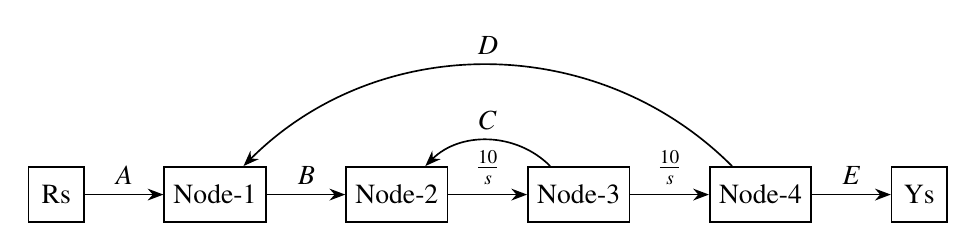
\begin{tikzpicture}[>=Stealth,auto,node distance=1cm,semithick]
  \tikzstyle{block}=[draw, fill=white, rectangle, minimum height=2em, minimum width=2em]
  
  \node [block] (input) {R\brak{s}};
  \node [block, right=of input] (filter) {Node-1};
  \node [block, right=of filter] (D) {Node-2};
  \node [block, right=of D] (E) {Node-3};
  \node [block, right=of E] (F) {Node-4};
  \node [block, right=of F] (output) {Y\brak{s}};
  
  \draw [->] (input) -- node {$A$} (filter);
  \draw [->] (filter) -- node {$B$} (D);
  \draw [->] (D) -- node {$\frac{10}{s}$} (E);
  \draw [->] (E) -- node {$\frac{10}{s}$} (F);
  \draw [->] (F) -- node {$E$} (output);
  
  % Backward loops
  \draw [->] (E) edge [bend right=45] node[above] {$C$} (D);
  \draw [->] (F) edge [bend right=45] node[above] {$D$} (filter);
\end{tikzpicture}%
}
\caption{Signal Flow Diagram}
\label{fig:your_label}
\end{figure}


Mason's Gain Formula is given by :
\begin{align}
    H\brak{s} = \sum_{i=1}^{N}\brak{\frac{P_i \Delta_i}{\Delta}} \label{eq:eq1_ee39}
\end{align}
\begin{table}[!ht] 
\centering
\setlength{\extrarowheight}{8pt}
\begin{tabular}{|l|l|}
    \hline
    \textbf{Parameter} & \textbf{Description}\\
    \hline
     N & Number of forward paths \\\hline
     L & Number of loops\\\hline
     $P_k$ & Forward path gain of $k^{th}$ path\\\hline
     $\Delta_k$ & Associated path factor \\\hline
     $\Delta$ & Determinant of the graph \\\hline
  \end{tabular}
  \vspace{4mm}
 \caption{Parameter Table - Mason's Gain Law}
 \label{tab:table1_ee_22_39}
\end{table}

\begin{table}[!ht] 
\centering
\setlength{\extrarowheight}{8pt}
\begin{tabular}{|l|l|}
    \hline
    \textbf{Parameter} & \textbf{Formula}\\
    \hline
     $\Delta$ & 1 + $\sum_{k=1}^{L}\brak{\brak{-1}^k\text{Product of gain of groups of k isolated loops}}$ \\\hline
     $\Delta_k$ & $\Delta$ part of graph that is not touching $k^{th}$ forward path \\\hline
  \end{tabular}
  \vspace{4mm}
 \caption{Formula Table - Mason's Gain Law}
 \label{tab:table2_ee_22_39}
\end{table}

This signal flow graph has only one forward path whose gain is given by :
\begin{align}
    P_1 &= \frac{10}{s} \frac{10}{s}\\
    &= \frac{100}{s^2}
\end{align}
The loop gain for loop between Node-2 and Node-3 is :
\begin{align}
    L_1 &= \frac{10}{s}\brak{-1}\\
    &= -\frac{10}{s}
\end{align}
The loop gain for loop between Node-1 and Node-4 is :
\begin{align}
    L_1 &= \frac{10}{s}\frac{10}{s}\brak{-1}\\
    &= -\frac{100}{s^2}
\end{align}
Using \tabref{tab:table2_ee_22_39}, $\Delta$ is :
\begin{align}
    \Delta &= 1 - \brak{-\frac{10}{s} - \frac{100}{s^2}}\\
    &= 1 + \frac{10}{s} + \frac{100}{s^2}
\end{align}
There are no two isolated loops available. Hence all further terms will b zero.\\
As both the loops are in contact with the only forward path,
\begin{align}
    \Delta_1 = 1
\end{align}
Using equation \eqref{eq:eq1_ee39} :
\begin{align}
    H\brak{s} &= \frac{\frac{100}{s^2}}{1 + \frac{10}{s} + \frac{100}{s^2}} \\
    &= \frac{100}{s^2 + 10s + 100}\label{eq:eq2_ee39}
\end{align}
Referring to \tabref{tab:table0_ee_22_39}, the general equation of the damping system is second order and can be written as :
\begin{align}
    m\ddot{y}(t) + c\dot{y}(t) + ky(t) = x(t)
\end{align}
Take the Laplace transform and solve for $\frac{Y\brak{s}}{X\brak{s}}$ :
\begin{align}
    \frac{Y\brak{s}}{X\brak{s}} &= \frac{\omega_n^2}{s^2 + 2\zeta\omega_n s + \omega_n^2}\\
\implies H\brak{s} &= \frac{\omega_n^2}{s^2 + 2\zeta\omega_n s + \omega_n^2} \label{eq:eq3_ee39}
\end{align}
Comparing equations \eqref{eq:eq2_ee39} and \eqref{eq:eq3_ee39} ,
\begin{align}
    \omega_n ^2 &= 100\\
    \implies \omega_n &= 10 \text{ rad/s} \label{eq:eq4_ee39}\\
    2\zeta \omega_n &= 10\\
    \implies \zeta &= 0.5
\end{align}
\begin{figure}[!ht]
\centering
\begin{center}
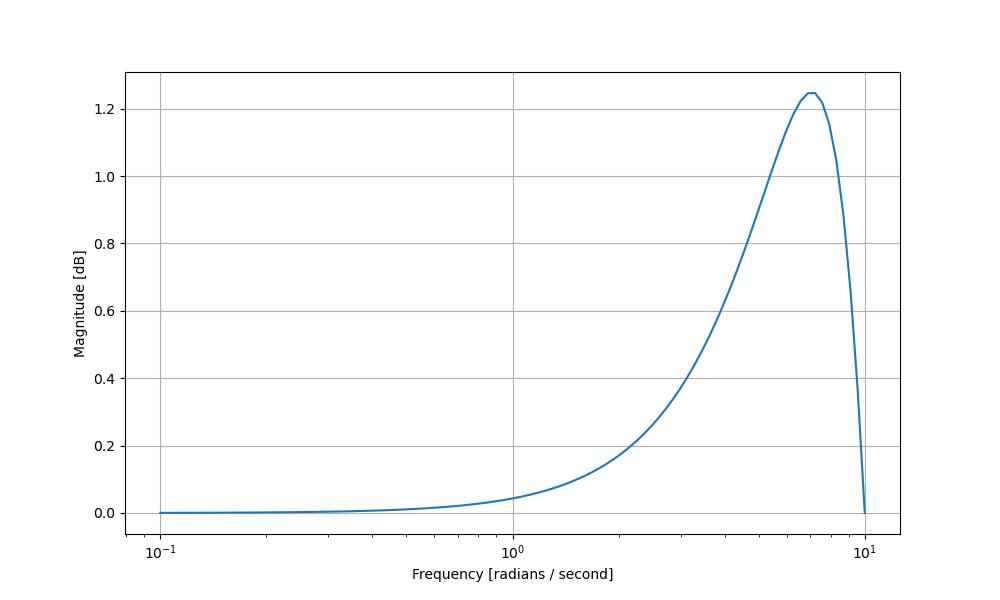
\includegraphics[width=\columnwidth]{2022/EE/39/figs/Figure_1.jpg}
\end{center}
\caption{Magnitude plot}
\end{figure}
\begin{figure}[!ht]
\centering
\begin{center}
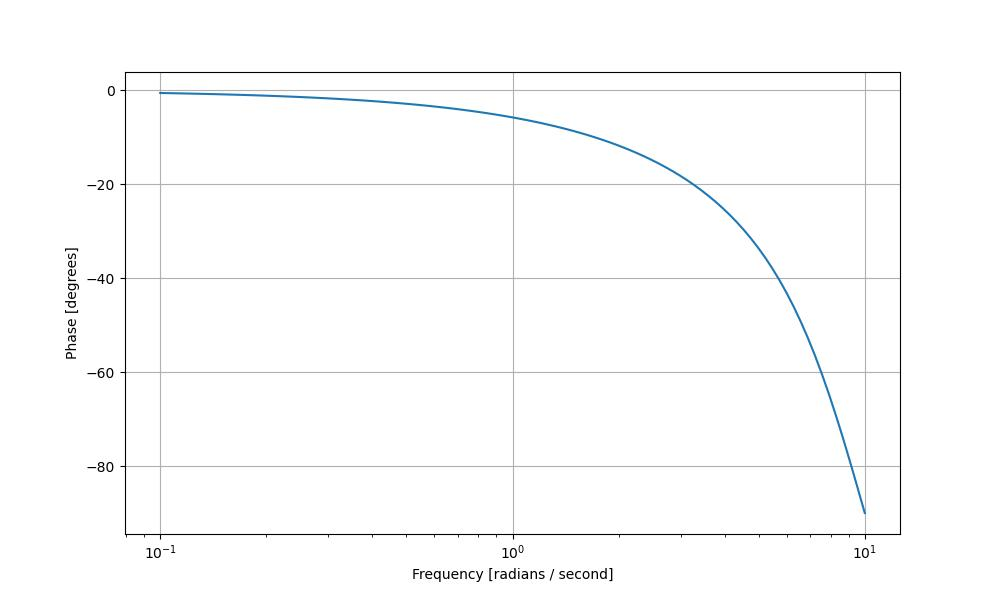
\includegraphics[width=\columnwidth]{2022/EE/39/figs/Figure_2.jpg}
\end{center}
\caption{Phase plot}
\end{figure}

\newpage
\item In the block diagram shown in the figure, the transfer function $G=\frac{K}{\tau s+1}$ with $K>0$ and $\tau>0$. The maximum value of $K$ below which the system remains stable is \rule{1cm}{0.15mm}(rounded off to two decimal places) \hfill (GATE CH 2022) 
\begin{figure}[htbp] 
\includegraphics[width=\columnwidth]{2022/CH/58/figs/question.jpg} 
\end{figure}\\ 
\solution 
\input{2022/CH/58/ch_58.tex} 
\newpage
\item The signal flow graph of a system is shown. The expression for $\frac{Y\brak{s}}{X\brak{s}}$ is
\begin{figure}[h]
    \centering
    \begin{tikzpicture}
    \draw (0,0) arc (0:360:0.1);
    \draw [->] (0,0) -- (2,0);
    \draw (2.2,0) arc (0:360:0.1);
    \draw [->] (2.2,0) -- (4.2,0);
    \draw (4.4,0) arc (0:360:0.1);
    \draw [->] (4.4,0) -- (6.4,0);
    \draw (6.6,0) arc (0:360:0.1);
    \draw (-0.5,0) node[below] {$X\brak{s}$};
    \draw (1.1, 0) node[above] {$G_1\brak{s}$};
    \draw (3.3,0) node[above]  {$G_2\brak{s}$};
    \draw (5.3, 0) node[above] {$2$};
    \draw (6.9,0) node[below] {$Y\brak{s}$};
    \draw [<-](4.3,0.1) arc (0:180:1.1);
    \draw [<-] (2.1, -0.1) arc (-180:0:1.1);
    \draw  (3.2,1.3) node[above] {$G_3\brak{s}$};
    \draw (3.2,-1.2) node[below] {-1};
    \draw (2,-0.3) node[left] {$a$};
    \draw (4.3, -0.3) node[right] {$b$};
    \end{tikzpicture}
    \caption{Signal Flow Graph of the System}
    \label{fig:sfg_in-37-2022}
\end{figure}
\begin{enumerate}[label=(\alph*)]
    \item $\frac{2 G_1\brak{s} G_2\brak{s} + 2 G_1\brak{s} G_3\brak{s} }{ 1 + G_2\brak{s} + G_3\brak{s} }$
    \item $ 2 + G_1\brak{s} + G_3\brak{s} + \frac{G_2\brak{s} }{ 1 + G_2\brak{s}}$
    \item $G_1\brak{s} + G_3\brak{s} - \frac{G_2\brak{s} }{ 2 + G_2\brak{s} }$
    \item $\frac{ 2 G_1\brak{s} G_2\brak{s} + 2 G_1\brak{s} G_3\brak{s} - G_1\brak{s} }{ 1 + G_2\brak{s} + G_3\brak{s} }$
\end{enumerate}\hfill(GATE 2022 IN Question 37) \\
\solution
\iffalse
\let\negmedspace\undefined
\let\negthickspace\undefined
\documentclass[journal,12pt,twocolumn]{IEEEtran}
\usepackage{cite}
\usepackage{amsmath,amssymb,amsfonts,amsthm}
\usepackage{algorithmic}
\usepackage{graphicx}
\usepackage{textcomp}
\usepackage{xcolor}
\usepackage{txfonts}
\usepackage{listings}
\usepackage{enumitem}
\usepackage{mathtools}
\usepackage{gensymb}
\usepackage{comment}
\usepackage[breaklinks=true]{hyperref}
\usepackage{tkz-euclide} 
\usepackage{listings}
\usepackage{gvv}                                        
\def\inputGnumericTable{}                                 
\usepackage[latin1]{inputenc}                                
\usepackage{color}                                            
\usepackage{array}                                            
\usepackage{longtable}                                       
\usepackage{calc}                                             
\usepackage{multirow}                                         
\usepackage{hhline}                                           
\usepackage{ifthen}                                           
\usepackage{lscape}
\newtheorem{theorem}{Theorem}[section]
\newtheorem{problem}{Problem}
\newtheorem{proposition}{Proposition}[section]
\newtheorem{lemma}{Lemma}[section]
\newtheorem{corollary}[theorem]{Corollary}
\newtheorem{example}{Example}[section]
\newtheorem{definition}[problem]{Definition}
\newcommand{\BEQA}{\begin{eqnarray}}
\newcommand{\EEQA}{\end{eqnarray}}
\newcommand{\define}{\stackrel{\triangle}{=}}
\theoremstyle{remark}
\newtheorem{rem}{Remark}
\begin{document}

\bibliographystyle{IEEEtran}
\vspace{3cm}

\title{IN-37}
\author{EE23BTECH11063 - Vemula Siddhartha}
\maketitle
\newpage
\bigskip

\renewcommand{\thefigure}{\theenumi}
\renewcommand{\thetable}{\theenumi}
\textbf{Question}:\\
The signal flow graph of a system is shown. The expression for $\frac{Y\brak{s}}{X\brak{s}}$ is
\begin{figure}[h]
    \centering
    \begin{tikzpicture}
    \draw (0,0) arc (0:360:0.1);
    \draw [->] (0,0) -- (2,0);
    \draw (2.2,0) arc (0:360:0.1);
    \draw [->] (2.2,0) -- (4.2,0);
    \draw (4.4,0) arc (0:360:0.1);
    \draw [->] (4.4,0) -- (6.4,0);
    \draw (6.6,0) arc (0:360:0.1);
    \draw (-0.5,0) node[below] {$X\brak{s}$};
    \draw (1.1, 0) node[above] {$G_1\brak{s}$};
    \draw (3.3,0) node[above]  {$G_2\brak{s}$};
    \draw (5.3, 0) node[above] {$2$};
    \draw (6.9,0) node[below] {$Y\brak{s}$};
    \draw [<-](4.3,0.1) arc (0:180:1.1);
    \draw [<-] (2.1, -0.1) arc (-180:0:1.1);
    \draw  (3.2,1.3) node[above] {$G_3\brak{s}$};
    \draw (3.2,-1.2) node[below] {-1};
    \draw (2,-0.3) node[left] {$a$};
    \draw (4.3, -0.3) node[right] {$b$};
    \end{tikzpicture}
    \caption{Signal Flow Graph of the System}
    \label{fig:sfg_in-37-2022}
\end{figure}
\begin{enumerate}[label=(\alph*)]
    \item $\frac{2 G_1\brak{s} G_2\brak{s} + 2 G_1\brak{s} G_3\brak{s} }{ 1 + G_2\brak{s} + G_3\brak{s} }$
    \item $ 2 + G_1\brak{s} + G_3\brak{s} + \frac{G_2\brak{s} }{ 1 + G_2\brak{s}}$
    \item $G_1\brak{s} + G_3\brak{s} - \frac{G_2\brak{s} }{ 2 + G_2\brak{s} }$
    \item $\frac{ 2 G_1\brak{s} G_2\brak{s} + 2 G_1\brak{s} G_3\brak{s} - G_1\brak{s} }{ 1 + G_2\brak{s} + G_3\brak{s} }$
\end{enumerate}\hfill(GATE 2022 IN Question 37) \\
\solution
\fi
\begin{table}[h!]    
    \centering
    \begin{tabular}{|c|c|c|}
    \hline
    \textbf{Parameter} & \textbf{Description} & \textbf{Value}\\ \hline
    $Y\brak{s}$ & Output node variable &\\
    \hline
    $X\brak{s}$ & Input node variable &\\
    \hline
    $\frac{Y\brak{s}}{R\brak{s}}$ & Transfer function & ?\\
    \hline
    $P_1$ & Forward Path Gain a-b through $G_2\brak{s}$ & $ 2 G_1\brak{s} G_2\brak{s} $ \\
    \hline
    $P_2$ & Forward Path Gain a-b through $G_3\brak{s}$ & $ 2 G_1\brak{s} G_3\brak{s}$ \\
    \hline
    $\Delta_1$ & Determinant of Forward Path a-b through $G_2\brak{s}$ & $1$ \\
    \hline
    $\Delta_2$ & Determinant of Forward Path a-b through $G_3\brak{s}$ & $1$ \\
    \hline
    $L_1$ & Gain of Loop a-b through $G_2\brak{s}$ and back & $-G_2\brak{s}$ \\
    \hline
    $L_2$ & Gain of Loop a-b through $G_3\brak{s}$ and back & $-G_3\brak{s}$ \\
    \hline 
    $\Delta$ & Determinant of System & $1+G_2\brak{s}+G_3\brak{s}$ \\
    \hline
    $n$ & Number of forward paths & $2$ \\
    \hline
    \end{tabular}
    \caption{Variables Used}
  \end{table}\\
  \begin{align}
    P_1 &= \brak{G_1\brak{s}} \brak{G_2\brak{s}} \brak{2} = 2 G_1\brak{s} G_2\brak{s} \\
    P_2 &= \brak{G_1\brak{s}} \brak{G_3\brak{s}} \brak{2} = 2 G_1\brak{s} G_3\brak{s} \\
    \Delta_1 &= 1 - \brak{0} = 1 \\
    \Delta_2 &= 1 - \brak{0} = 1 \\
    L_1 &= -G_2\brak{s} \\
    L_2 &= -G_3\brak{s} \\
    \Delta &= 1 - \brak{L_1 + L_2} = 1 + G_1\brak{s} + G_2\brak{s}
  \end{align}
  From \ref{fig:sfg_in-37-2022}, Using Mason's Gain Formula,
  \begin{align}
    \frac { Y\brak{s} }{ X\brak{s} } &= \frac { \sum_{ i = 1 }^{ n } P_i \Delta_i } { \Delta } \\
    &= \frac { P_1 \Delta_1 + P_2 \Delta_2 } { \Delta } \\
    &= \frac { 2 G_1\brak{s} G_2 \brak{s} \brak{1} + 2 G_1\brak{s} G_3\brak{s} \brak{1} } { 1 + G_2\brak{s} + G_3\brak{s} } \\
    \implies \frac { Y\brak{s} }{ X\brak{s} } &= \frac { 2 G_1\brak{s} G_2\brak{s} + 2 G_1\brak{s} G_3\brak{s} } { 1 + G_2\brak{s} + G_3\brak{s} }
  \end{align}

\newpage
\end{enumerate}
